\documentclass[11pt]{article}
\usepackage{graphicx}
\usepackage{hyperref}
\usepackage[letterpaper, portrait, margin=1in]{geometry}
\usepackage{fancyhdr}
\usepackage{pdfpages}
\usepackage{color}

\usepackage{charter}
\pagestyle{fancy}
\lhead{SURFv5 documentation}
%\chead{\thepage}
\rhead{v.0.1 ---  2016/9/16}


%\usepackage{lmodern}

\begin{document}
\noindent Authors: Eric Oberla (UChicago), 

\tableofcontents
\newpage

\section{Overview}

This document provides a brief overview of operating the SURFv5 circuit board based on the LAB4D waveform sampling ASIC. The SURFv5 board was designed by Patrick Allison (OSU) and Jarred Roberts (UHawai'i). The LAB4D ASIC was designed by Gary Varner (UHawai'i). P. Allison developed the FPGA firmware. Testing of this hardware began in June, 2016. This work is part of the ANITA project.

The SURFv5 board, pictured in Fig.~\ref{fig:surf}, houses 12 LAB4D ASICs corresponding to 12 RF channels. Each ASIC has only a single channel per chip to minimize channel-to-channel crosstalk via the IC package bondwires and/or on-die coupling. Each RF channel is equipped with a bandpass filter, nominally $\sim$140 - 1000 MHz\footnote{filters used: low pass is Mini-Circuits LFCN-1000+; high pass is Mini-Circuits HFCV-145+}. The SURFv5 front panel also has two `SYNC' inputs which are split and coupled onto the RF signal lines after the bandpass filter. The SYNC inputs pass baseband signals up to $\sim$250 MHz, which allows {\it in situ} time synching between channels/SURFs and the parallelization of the LAB4D timebase calibrations. 

For the ANITA mission, the plan is to run the LAB4D  at 3.2 GSa/s with 1024 samples-per-event (event record window $=$ 320 ns). The LAB4D has a total of 4096 samples, which allows the (analog) multi-buffering of four events and simultaneous read/write operation, reducing dead-time induced latency.

A key feature of the LAB4D ASIC is the ability to trim the inherently non-uniform time-base delays of a CMOS voltage-controlled delay line, reducing previously required calibration and processing overhead for these ASICs. A tuning procedure is included that has demonstrated a spread on the sampling intervals of a few picoseconds.

\begin{figure}[h!]
    \begin{center}
      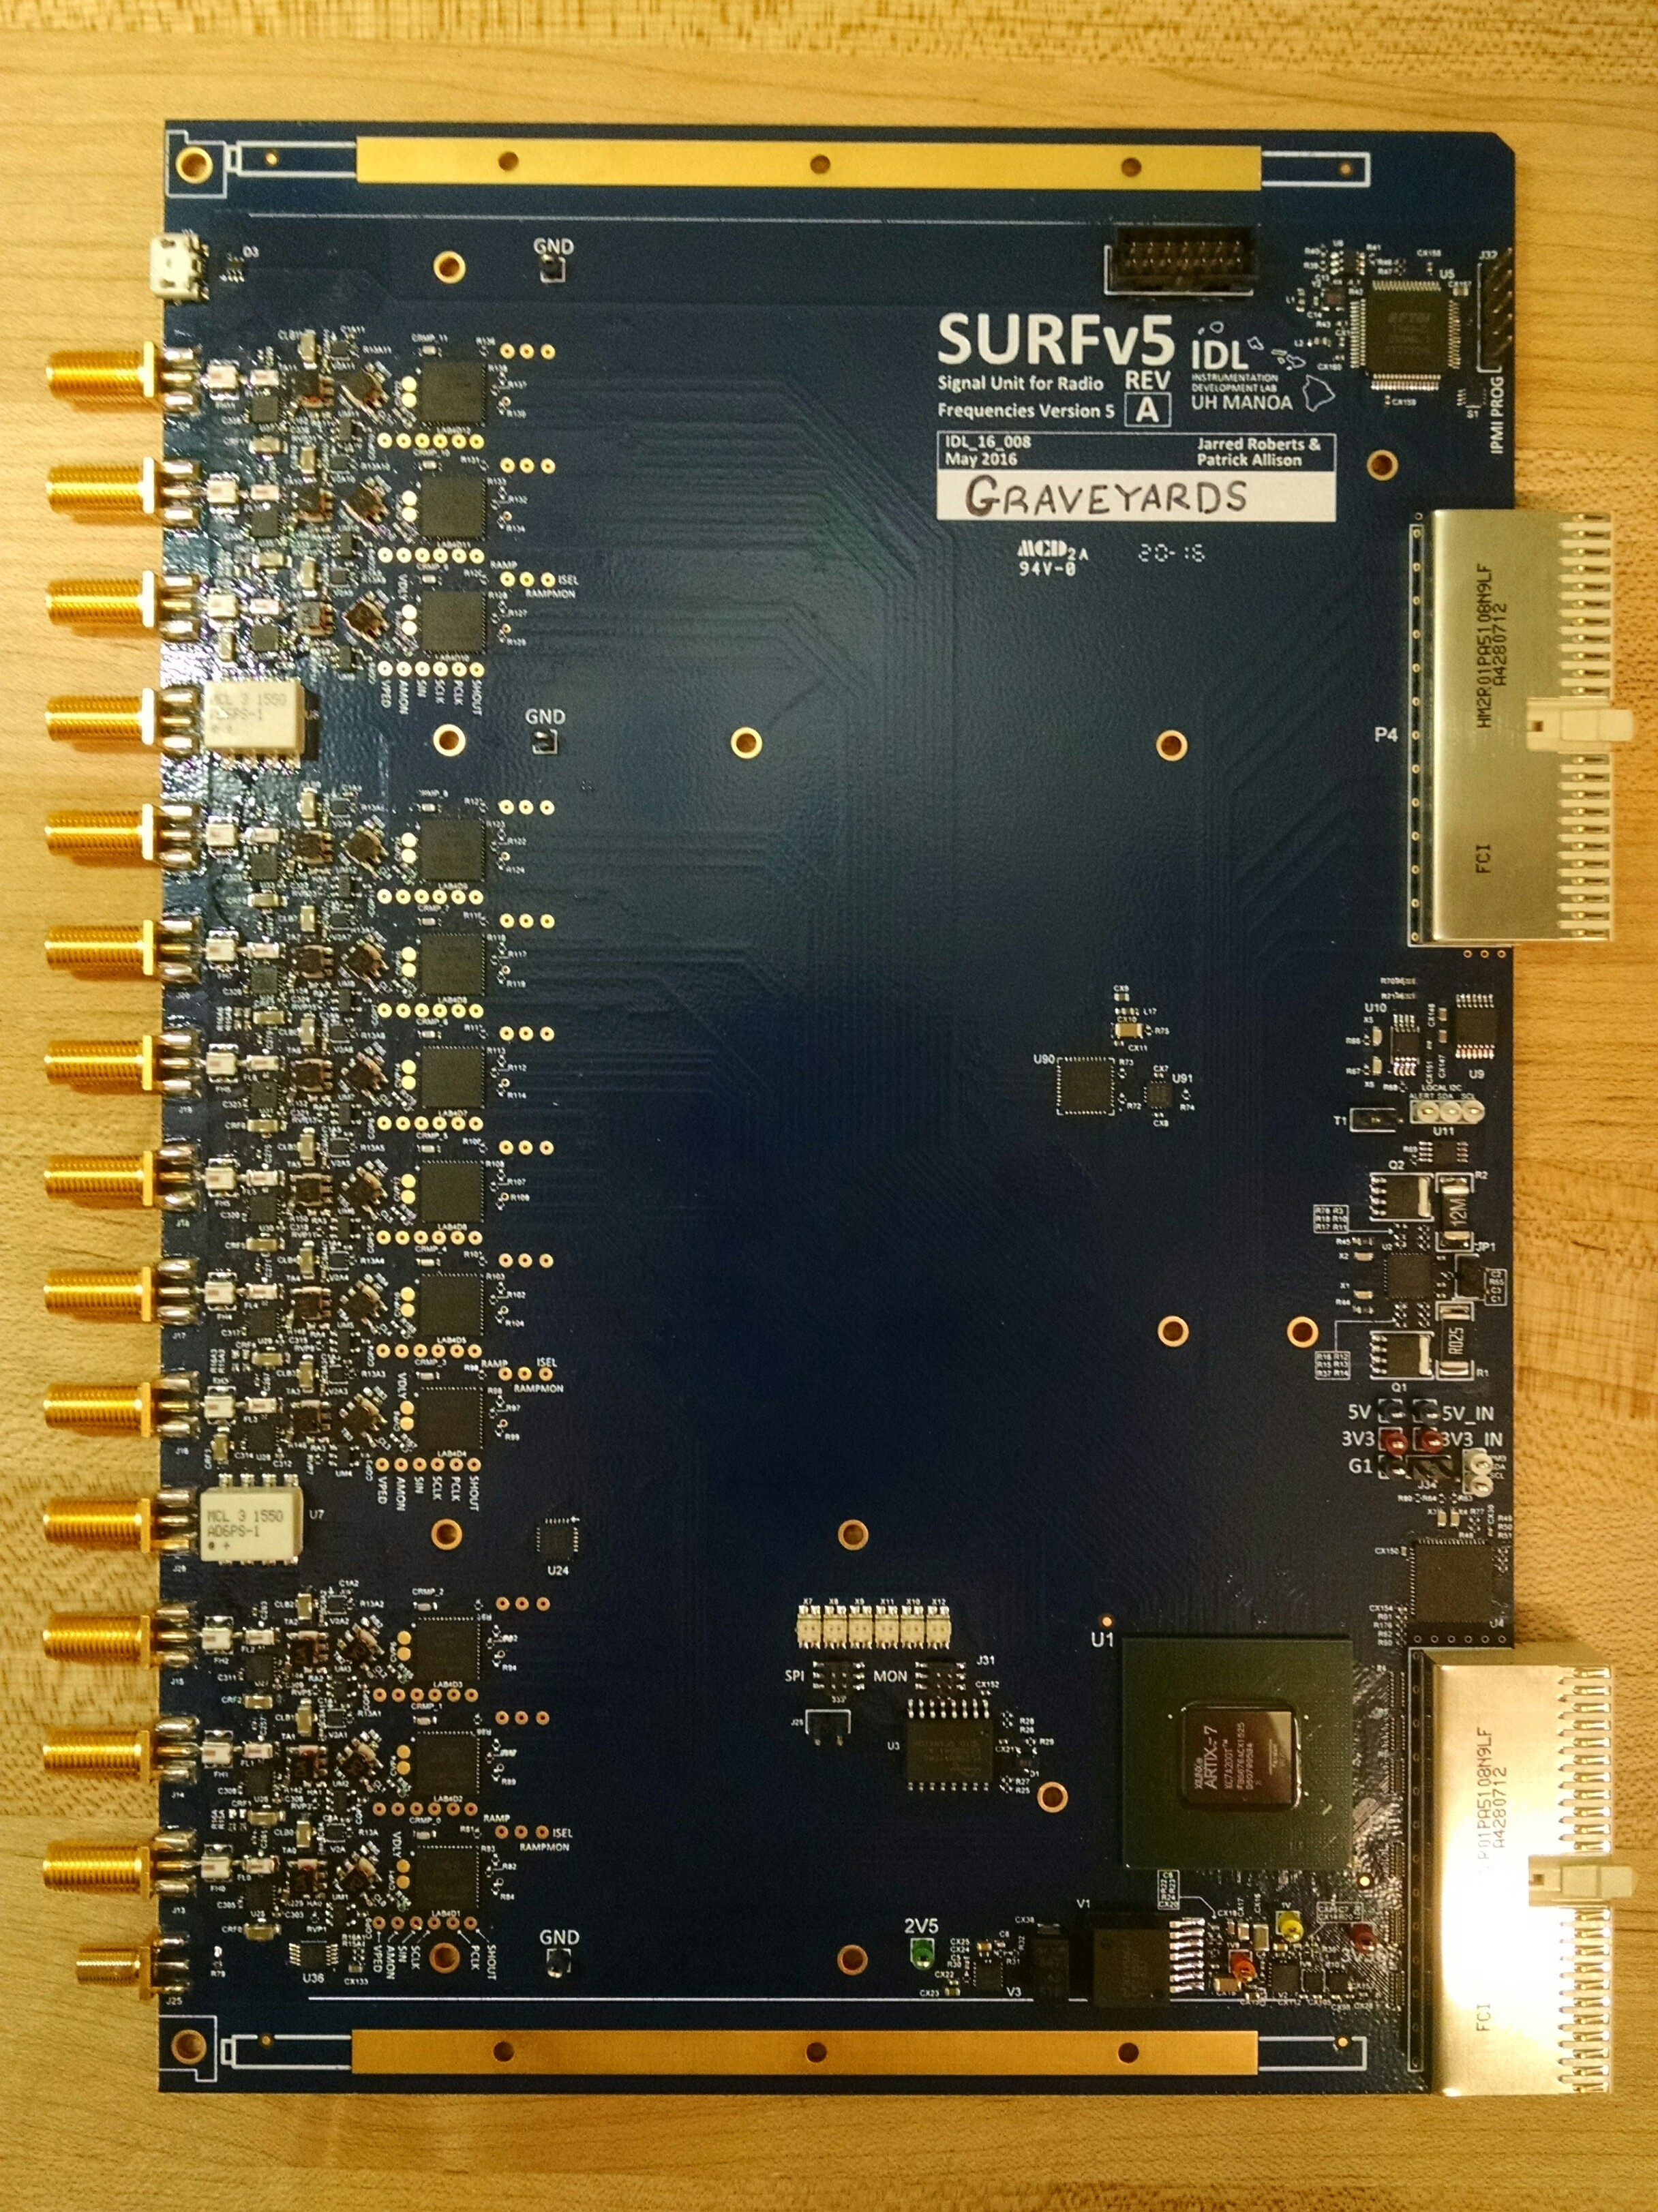
\includegraphics[width=10cm]{fig/graveyards.jpg}
      %\includegraphics[width=15cm]{singlePLL.PNG}

    \end{center}
    \caption{SURFv5 board (`GRAVEYARDS')}
    \label{fig:surf}
\end{figure}


\subsection{code respositories}
\label{code respositories}

\begin{itemize}
\item The firmware for the SURFv5 is available at P. Allison's github: \\\href{https://github.com/barawn/firmware-surf5}{https://github.com/barawn/firmware-surf5}

\item Python software for running a SURFv5 testbench can be found here: \\\href{https://github.com/ejobe/surf-pythoon}{https://github.com/ejobe/surf-python}
\end{itemize}
  
Notes about the Python sofware:
In the main directory, \verb!surf.py! and \verb!surf_data.py! are the main SURFv5 drivers. Subdirectory \verb!calibrations/! stores the \verb!surf_calibrations.json! cal file that holds channel-specific LAB4D register values as well as pedestal data, \verb!timing/! has the timebase-tuning modules. The file \verb!utils/surf_constants.py! defines a number of variables for the DAQ system as well as default values for the LAB4D registers. 


%%%%%%%%%%%%%%%%%%%%%%%%%%%%5
\section{Getting Started}

(Leaving out detailed instructions on how to program the FPGA. Either use a standard Xilinx cable and iMPACT loader or use \href{https://github.com/barawn/xvcd-anita}{P. Allison's nifty xcvd-anita daemon}. The latter, however, is currently unable to load the SPI flash device.)

\begin{enumerate}

\item
  {\bf Download the software linked above.} There's nothing really special here: You'll need some standard Python packages like numpy, json, matplotlib, and scipy installed.

\item
  {\bf Run surf\_board.py} This module sets up default configurations, enables the DLL, and does some basic calibrations if it's the first time the board has been operated. 

  To run: \verb!python surf_board.py [BoardName]!

  Alternatively this can be run in the Python interpreter:

  \verb!dev=surf_board.do(BoardName) #dev returns an instance of the Surf class!

  \smallskip
  where BoardName is the human-readable all-caps `surf break' identifier written on the board. This identifier is used to read/write to the surf\_calibrations.json file stored in \verb!calibrations/!.

\item {\bf Take pedestal data}. Save the fixed-pattern pedestal data to the \verb!surf_calibration.json! file. (Also see Appendix~\ref{Appendix1})

  To run: \verb!python surf_data.py pedestal!

  The pedestal data is also saved to an ascii file: \verb!calibrations/peds.temp! 

\item {\bf Check baseline waveforms} Check to see if pedestal-subtracted baseline looks OK. Many ways to do this; one option to use the `scope' option:
  
  \verb!python surf_data.py scope [Channel]!

  \smallskip
  where Channel is 0-11 (or if undefine will plot all channels). If data has spikes or an apparent RMS value above 10 ADC counts, re-run the pedestal calibration. (Also see Appendix~\ref{Appendix1})
  
\end{enumerate}


%%%%%%%%%%%%%%%%%%%%%%%%%%%
\section{Basic Operations}
A few DAQ operations are described here. These are shown in more detail within the IPython notebook attached in Appendix~\ref{Appendix1}:

\subsection*{setting the pedestal level}
The pedestal voltage is controlled with an I2C DAC. The pedestal level is accessed within the Surf class.

\verb!dev=surf.Surf()!

\verb!dev.vped  #prints pedestal level!

\verb!dev.set_vped(level)  #sets pedestal level!

\smallskip
where level is an integer between 0 and 4096.

\subsection*{saving/loading pedestal data}
Pedestal data can be taken from the command line (make sure no active signaling on the input!):

To run: \verb!python surf_data.py pedestal!

\smallskip
This runs the default 160 events to form the pedestal calibration data.

To read the pedestal data:

\verb!devData=surf_data.SurfData()!

\verb!devData.loadPed() #this calls calibrations.surf_calibrations.read_pedestals()!

\verb!ped = devData.pedestals #pedestals stored in class variable!


\subsection*{logging data}
Data are saved to a flat ascii file (12 columns, 1024*NumEvents rows). Data can be logged using:

\verb!python surf_data.py log [NumEvents] [filename]!

\subsection*{pedestal scan}
The DC transfer curve can be extracted by scanning the pedestal voltage generated by the on-board DAC:

\verb!python surf_data.py lin [Start] [Stop] [Interval]!

\smallskip
where Start is the DAC start code, Stop is the DAC stop code, and Interval is the scan interval.
If not provided, default values are used.

The SurfData class also has a function to create a channel-level LUT
based on the mean transfer function of all the storage cells. \textcolor{red}{TO-DO: implement per-storage-cell LUT (i.e. 4096 LUTs/LAB4D). Add option to apply this to readout.} 

%%%%%%%%%%%%%%%%%%%%%%%%%%%
\section{Calibrating the LAB4D Timebase}

The LAB4D ASIC has 128 primary sampling cells, which are toggled by an equivalent length voltage-controlled delay line. Due to the nature
of chip fabrication, these 128 sample intervals will have some variance around the nominal unit delay. The LAB4D is equipped with a trim DAC
on each delay cell to narrow the distribution of these sample intervals on-chip.
Additionally, the LAB4D has an on-chip delay-locked loop (DLL) that enables exactly one input clock period to traverse those 128 sample cells.
The DLL functionality enables synching between channels when broadcasting a common, low-jitter clock to all LAB4Ds.

In order to find the nominal parameters for tuning the timebase we first tune the DLL, which already provides quite good-looking waveform data. Further, we include
a process to tune the trim DACs to minimize the variation of the sample intervals. The process of tuning the DLL is a few orders of magnitude quicker than
tuning the sample intervals.

\subsection{Tuning the DLL feedback trim}

It is assumed that the DLL is enabled on the LAB4D, as it is in the \verb!surf_board.py! initialization script.
If not, call the \verb!dll(lab, mode=True)! function [\verb!lab!=15 to address all LABs on the board, otherwise specify 0-11] in the \verb!LAB4Controller! class in \verb!surf.py!.

There are primarily two parameters in the LAB4D register space that manage the tuning of the DLL: \verb!sstoutfb! and \verb!vtrimfb!.
\verb!sstoutfb! specifies the delay tap in the voltage-controlled delay line to phase-compare to the input reference clock. At the moment this is hard-coded
to \verb!sstoutfb! = 104. It is likely that this parameter needs to be uniquely set to 105 or 103 for specific LAB4D chips within the lot.

The DAC \verb!vtrimfb! sets the total amount of delay in the DLL by finely tuning the the delay of the \verb!sstoutfb! VCDL pick-off.
The optimal \verb!vtrimfb! can be found by scanning this parameter and fitting sine waves in groups of 128 cells corresponding to the primary sampling bank (i.e. excluding the DLL wraparound cells from the fit) at each \verb!vtrimfb! setting. The value is then extracted by comparing the fit results to the known input frequency and nominal sampling rate. Lower frequencies are better for this tuning: $\sim$100-230~MHz and advisably excluding multiples of 25~MHz, the input clock frequency.
To expediate the process, \verb!vtrimfb! can be incremented at intervals of $\sim$10 counts and fit with a 3rd or 4th order polynomial.

A function to tune the \verb!vtrimfb! parameter is given: \verb!timing/tune_dll_trim.py!.
An example on how to use this for tuning, saving, and loading trim values is given in Appendix~\ref{Appendix2}.

Figure~\ref{fig:fbsstout} shows the \verb!vtrimfb! tuning curves for \verb!sstoutfb! set to 104 and 105 on a single LAB4D.
We picked \verb!sstoutfb!=104 as it appears to give the widest stable range of tuning around the nominal sampling rate, 3.2 GSa/s.

Figure~\ref{fig:tunefb} shows multiple \verb!vtrimfb! taken during at differerent iterations during a VCDL-trim-DAC tuning run (described in next section).
The plot shows that the optimal value for \verb!vtrimfb! varies very little even when changing the VCDL trim-DAC values. 

\begin{figure}[h!]
  \begin{center}
    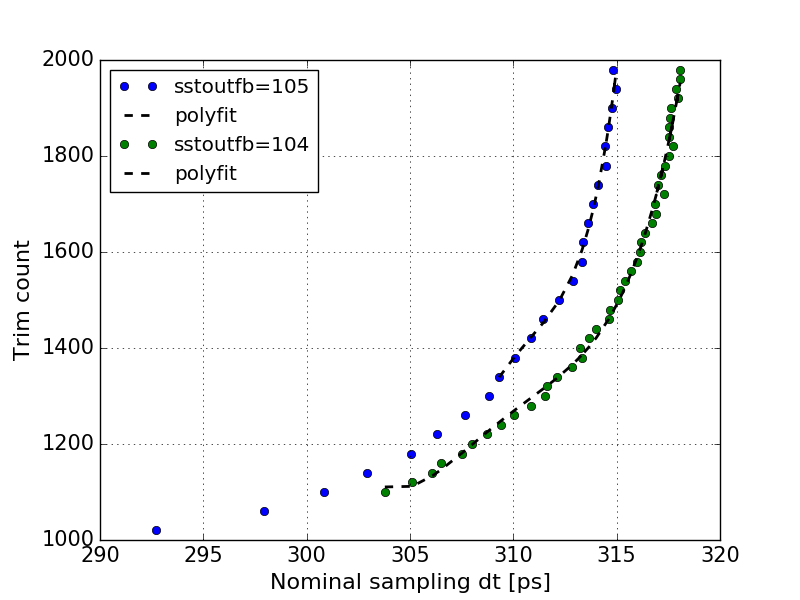
\includegraphics[width=11cm]{fig/fitVtrimFB_v2.png}
  \end{center}
  \caption{Scanning \texttt{vtrimfb} and fitting sine wave data to determine the optimal parameters for the DLL.}
  \label{fig:fbsstout}
\end{figure}


\begin{figure}[h!]
  \begin{center}
    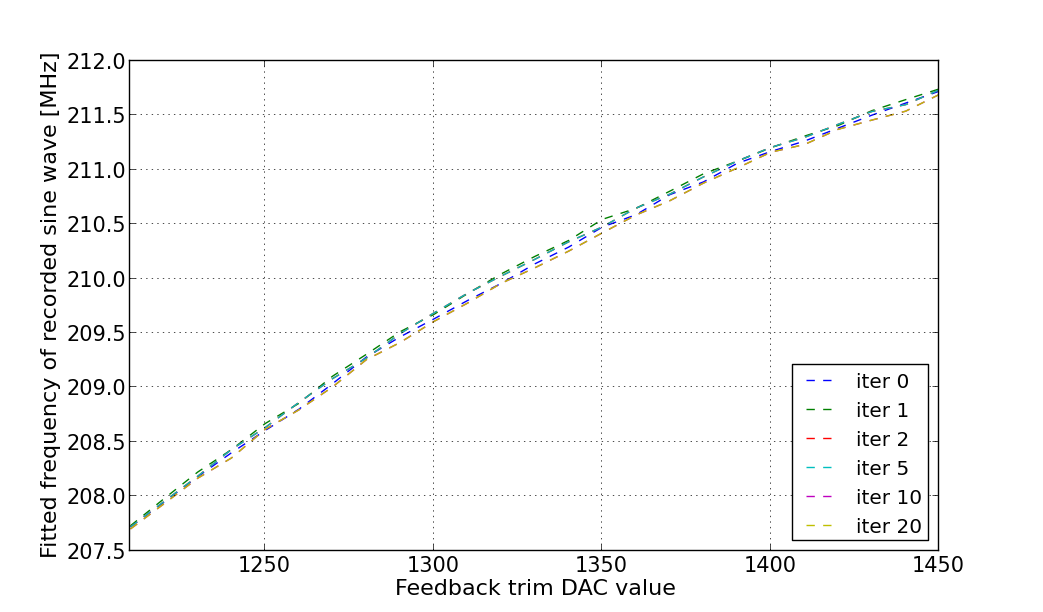
\includegraphics[width=15cm]{fig/fbTrimScan.png}
  \end{center}
  \caption{Fitted sine-wave frequency vs the feedback trim value using a 210.0 MHz sine-wave input on channel 0 of `CANOES'. The curve is robust against adjuments to the time-base trim dac values (next section) so presumably can just be calibrated once. [This measurement shows the turning curve at several iterations in the trim-dac tuning procedure.]}
  \label{fig:tunefb}
\end{figure}


\subsection{Tuning the VCDL trim DACs}

A straightforwared Newton's Method minimzation is currently used to tune the VCDL trim DACs. The functions are defined in \verb!timing/timing.py! and
an executable to run the minimization is \verb!timing/run_timing_cal.py!, which should be edited to specify the channels to tune, the number of iterations,
the output filename, and the number of events per iteration.

The minimazation curve used in this procedure is defined in \verb!timing/trim_minimization_curve.py!. It's mostly ad-hoc, but does the trick. The scheme
is based on low-statistics measurements of the individual trim-dac-value vs. sample-interval-time curve shown in Figure~\ref{fig:indivdttrim}


  \begin{figure}[h!]
  \begin{center}
    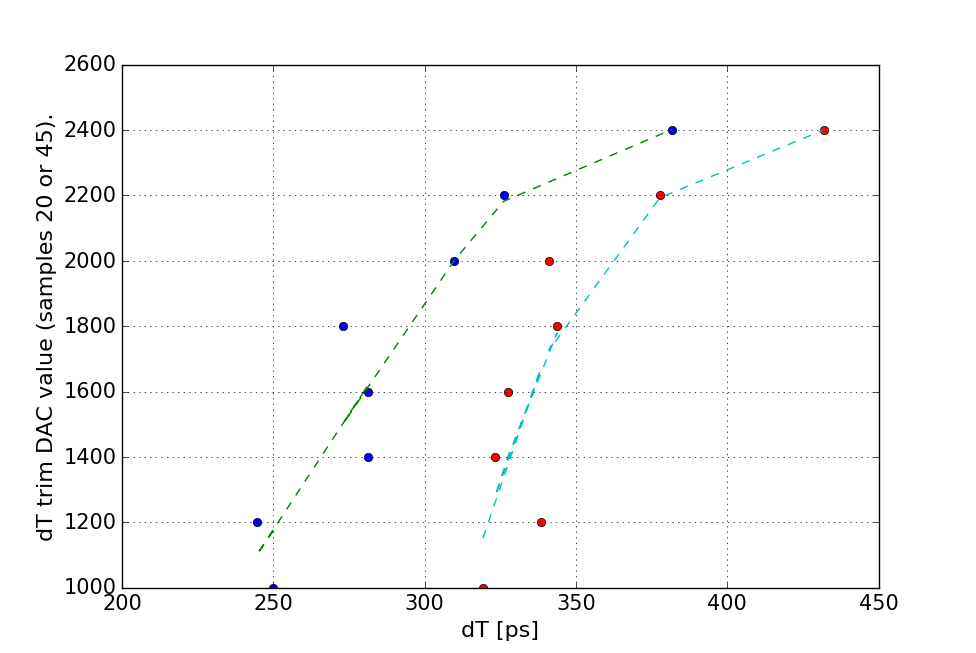
\includegraphics[width=12cm]{fig/dt_comparison_odd_even_cell.png}
  \end{center}
  \caption{dT trim DAC value vs. measured sampling interval for an even and odd sampling cell. }
  \label{fig:indivdttrim}
\end{figure}

The minimization method is based on counting the zero-crossings of sine-waves in the LAB4D data. The effective sampling interval is determined by
the relative occupancy in each sample-bin. At each iteration, the sampling interval is computed and the trim DAC is adjusted based on the minimization curve.
Because the zero-crossing method only uses a small amount of the total waveform around the zero-point, this method requires a large number of events. I have found
that 4000-8000 events per iteration (=32,000-64,000 passes at the primary sampling cells) yield a fairly robust result. Of course, higher statistics are always desired
and probably required to push down to the $\sim$ps level (though understanding the temperature dependence and the the linearity of the trim DACs become important issues at this point anyway).

Example results from a tuning run on Channel 0 of the SURFv5 called `CANOES' is shown in Fig~\ref{fig:tunetime}. The output of the tuning executable is a set of
.json files. In this run, the standard deviation of the sampling intervals
is pushed down to $\sim$2-3~ps (which is $< 1$\% on the nominal sampling rate!). A script is included to make these plots: \verb!timing/read_timing_json.py!

\begin{figure}[h!]
    \begin{center}
      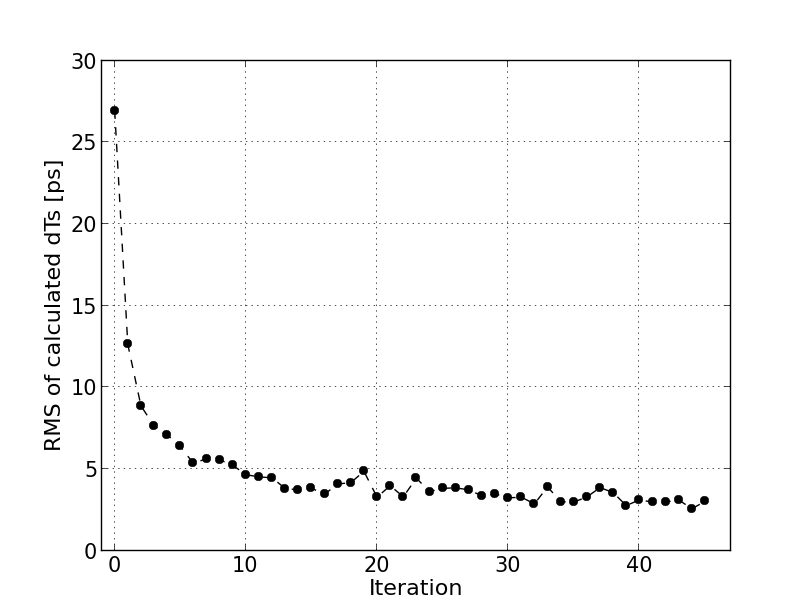
\includegraphics[width=8.2cm]{fig/RMSvsIter_919.png}
      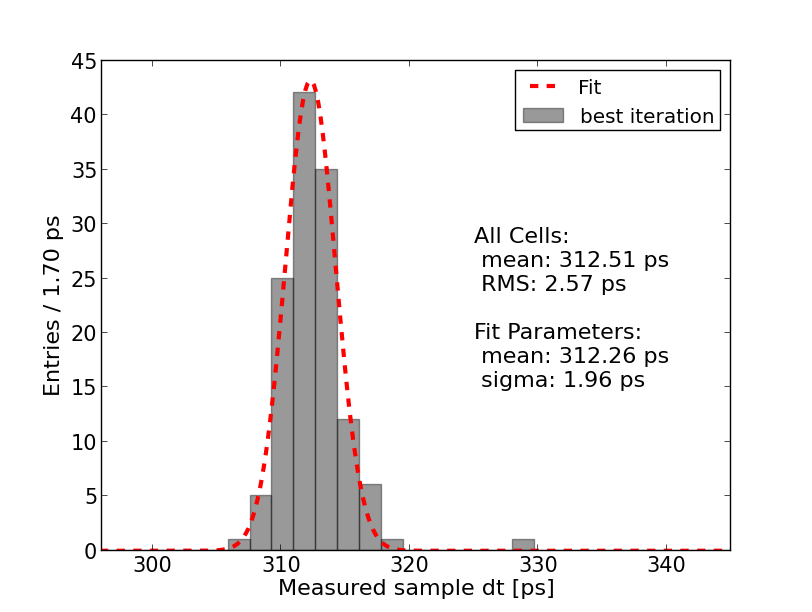
\includegraphics[width=8.2cm]{fig/dtHist_0919.png} \\
      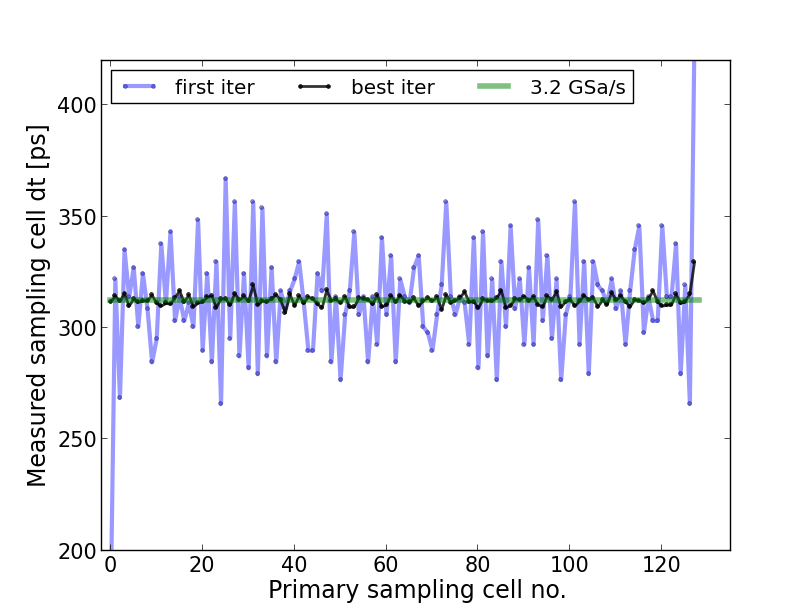
\includegraphics[width=8.2cm]{fig/dtDifferentialNonlinearity_0919.png}
      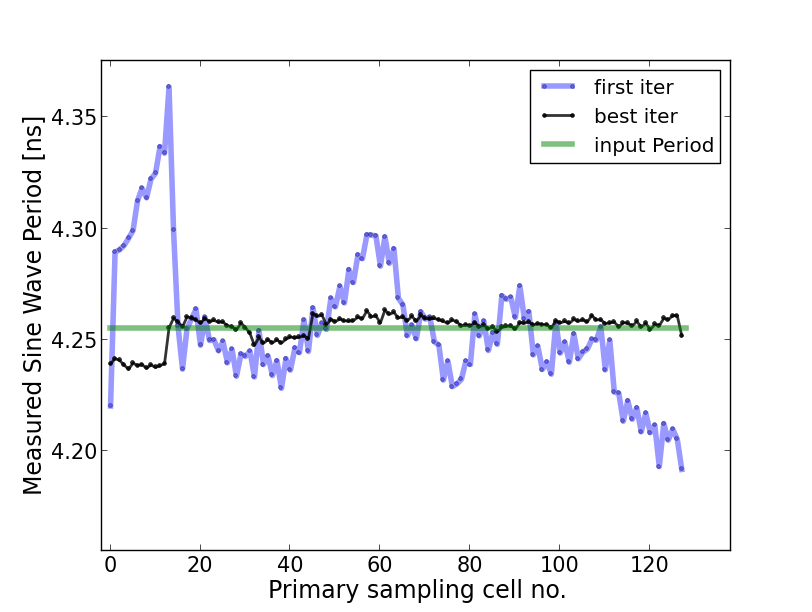
\includegraphics[width=8.2cm]{fig/periodIntegralNonlinearity_0919.png}
    \end{center}
    \caption{Timebase tuning results on Channel 0 of SURFv5 `CANOES' using 235.0 MHz sine wave.  Upper left: RMS vs iteration number.  Upper right: histogram of measured sampling intervals after tuning.  Lower left: Sampling interval at each interval before and after tuning (i.e. the Differential non-linearity) 
    Lower right: The measured periods using interpolated zero-crossings of before and after (i.e. getting at the integral non-linearity). }
    \label{fig:tunetime}
\end{figure}


\section{Analog Bandwidth}

The analog bandwidth of the SURFv5 (with a LCFN-1200+ low pass filter installed)  was measured using a 100~ps rise-and-fall time pulse. The width of this pulse was also about 100 ps.
The SURFv5 waveforms were averaged and windowed. A measurement of the analog bandwidth compared to the impulse measured on a commercial 2~GHz oscilloscope
is showsn in Fig.~\ref{fig:bwplots}. The small signal bandwidth is approximately 1.1~GHz~\footnote{It appears the SURFv5 bandwidth will be limited by the on-board filters not by the LAB4D input parasitics,
  so once the correct 1~GHz low pass is installed the high-end bandwidth will drop accordingly}

This should not be considered an exhaustive look at the frequency response of the SURFv5's or LAB4D chips.
\begin{figure}[h!]
    \begin{center}
      %%\includegraphics[width=8.2cm]{fig/bandwidth_impulse.png}
      \hspace{10pt}
      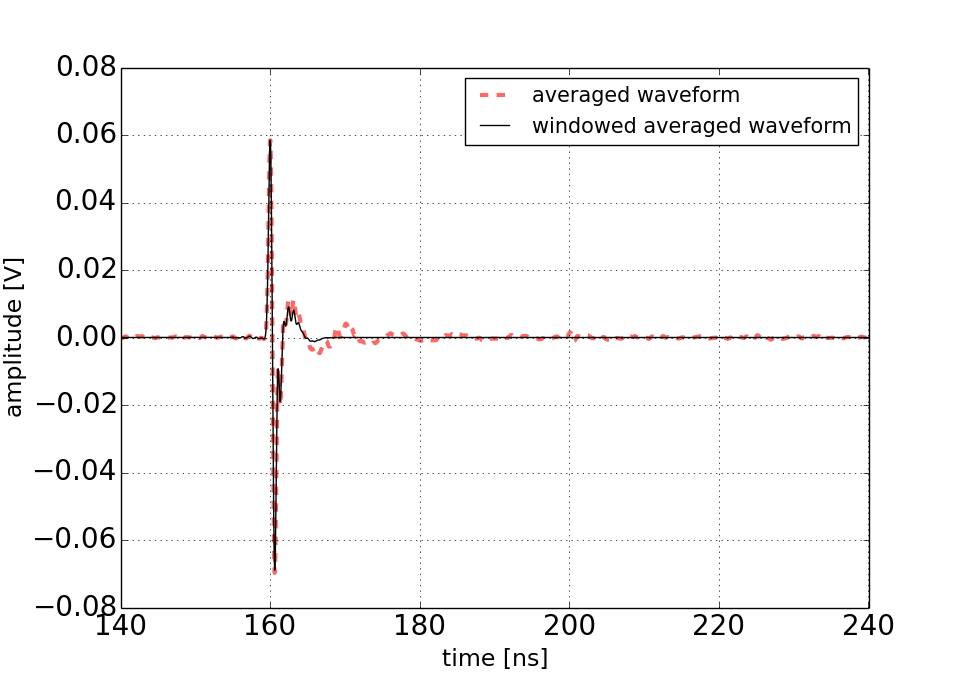
\includegraphics[width=11cm]{fig/bandwidth_waveforms.png} \\
      %%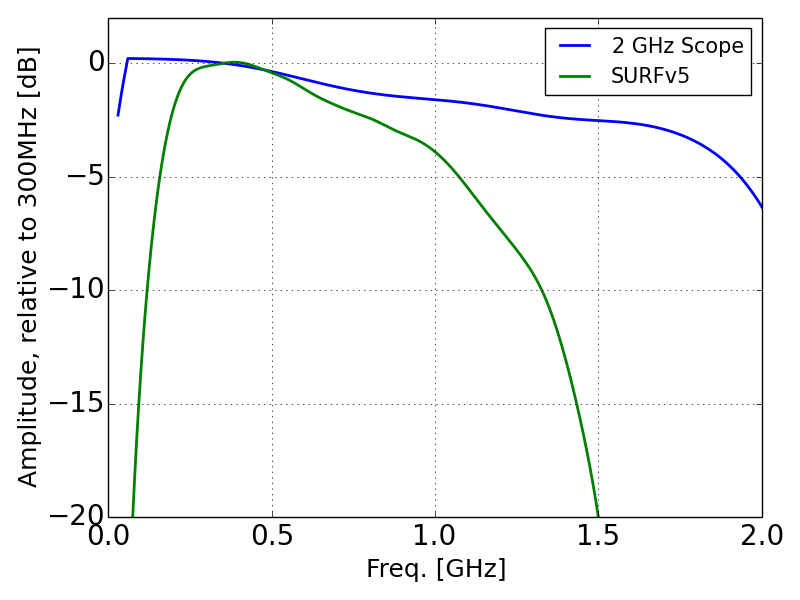
\includegraphics[width=8.2cm]{fig/bandwidth_compare.png} \\
      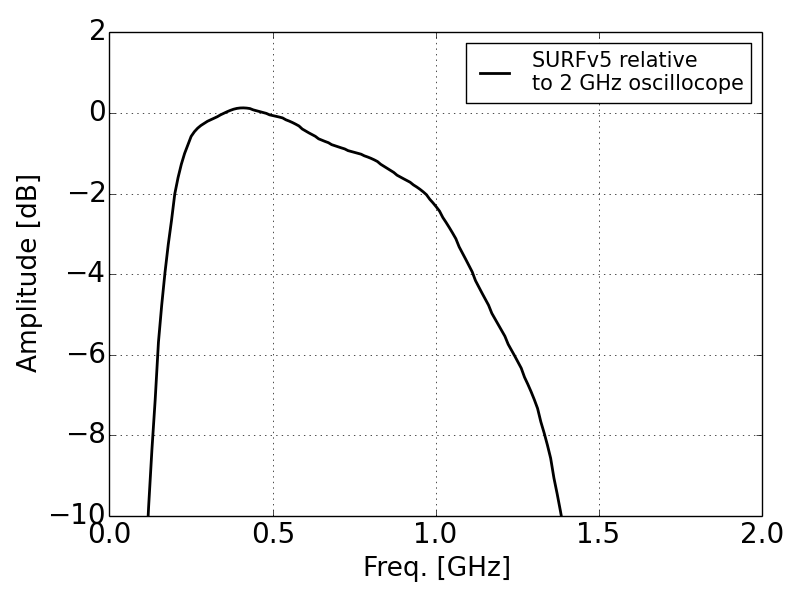
\includegraphics[width=11cm]{fig/bandwidth_surfV5.png}
    \end{center}
    \caption{Averaged recorded waveform from a $\sim$100~ps rise-time impulse and resultant (small-signal) bandwidth measurement (Channel 0 of SURFv5 `CANOES')}
    \label{fig:bwplots}
\end{figure}



\clearpage

\appendix

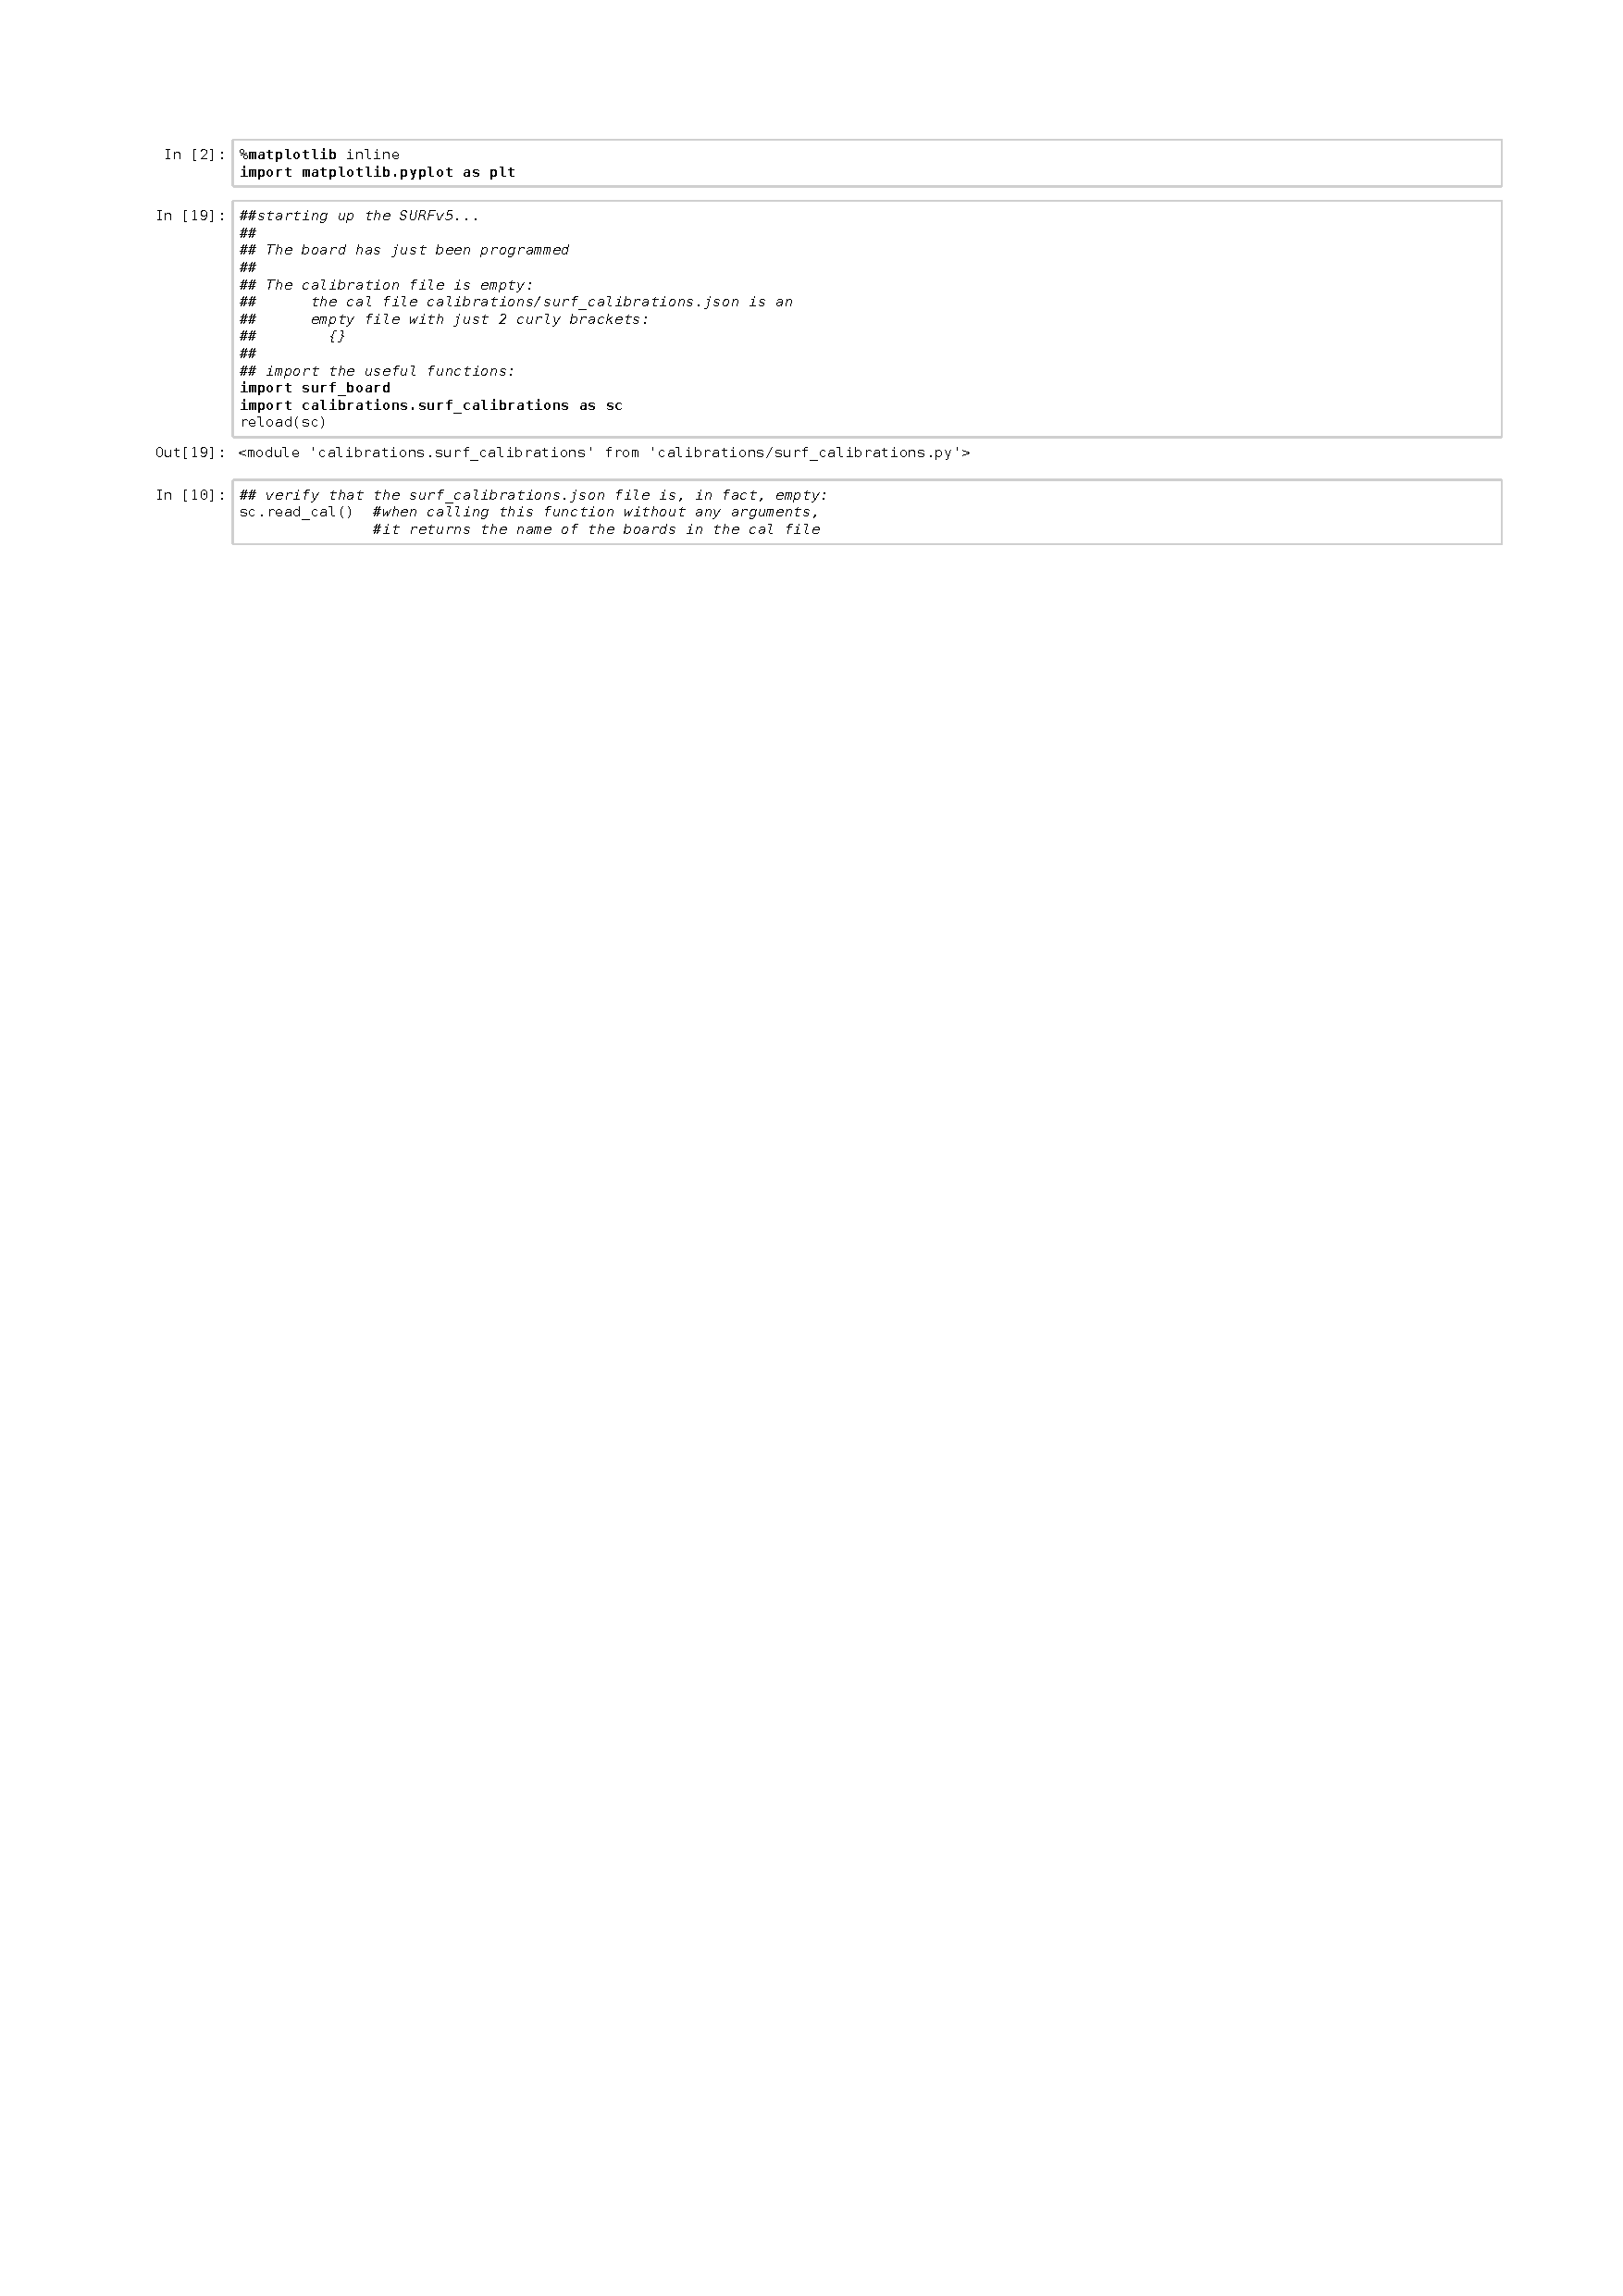
\includepdf[pages={1},  offset=0cm -6cm, pagecommand={\section{IPython Notebook: Startup}\label{Appendix0}}]{fig/bootSurf_notebook.pdf}
\includepdf[pages=2-, offset=0cm -1cm, pagecommand={}]{fig/bootSurf_notebook.pdf}

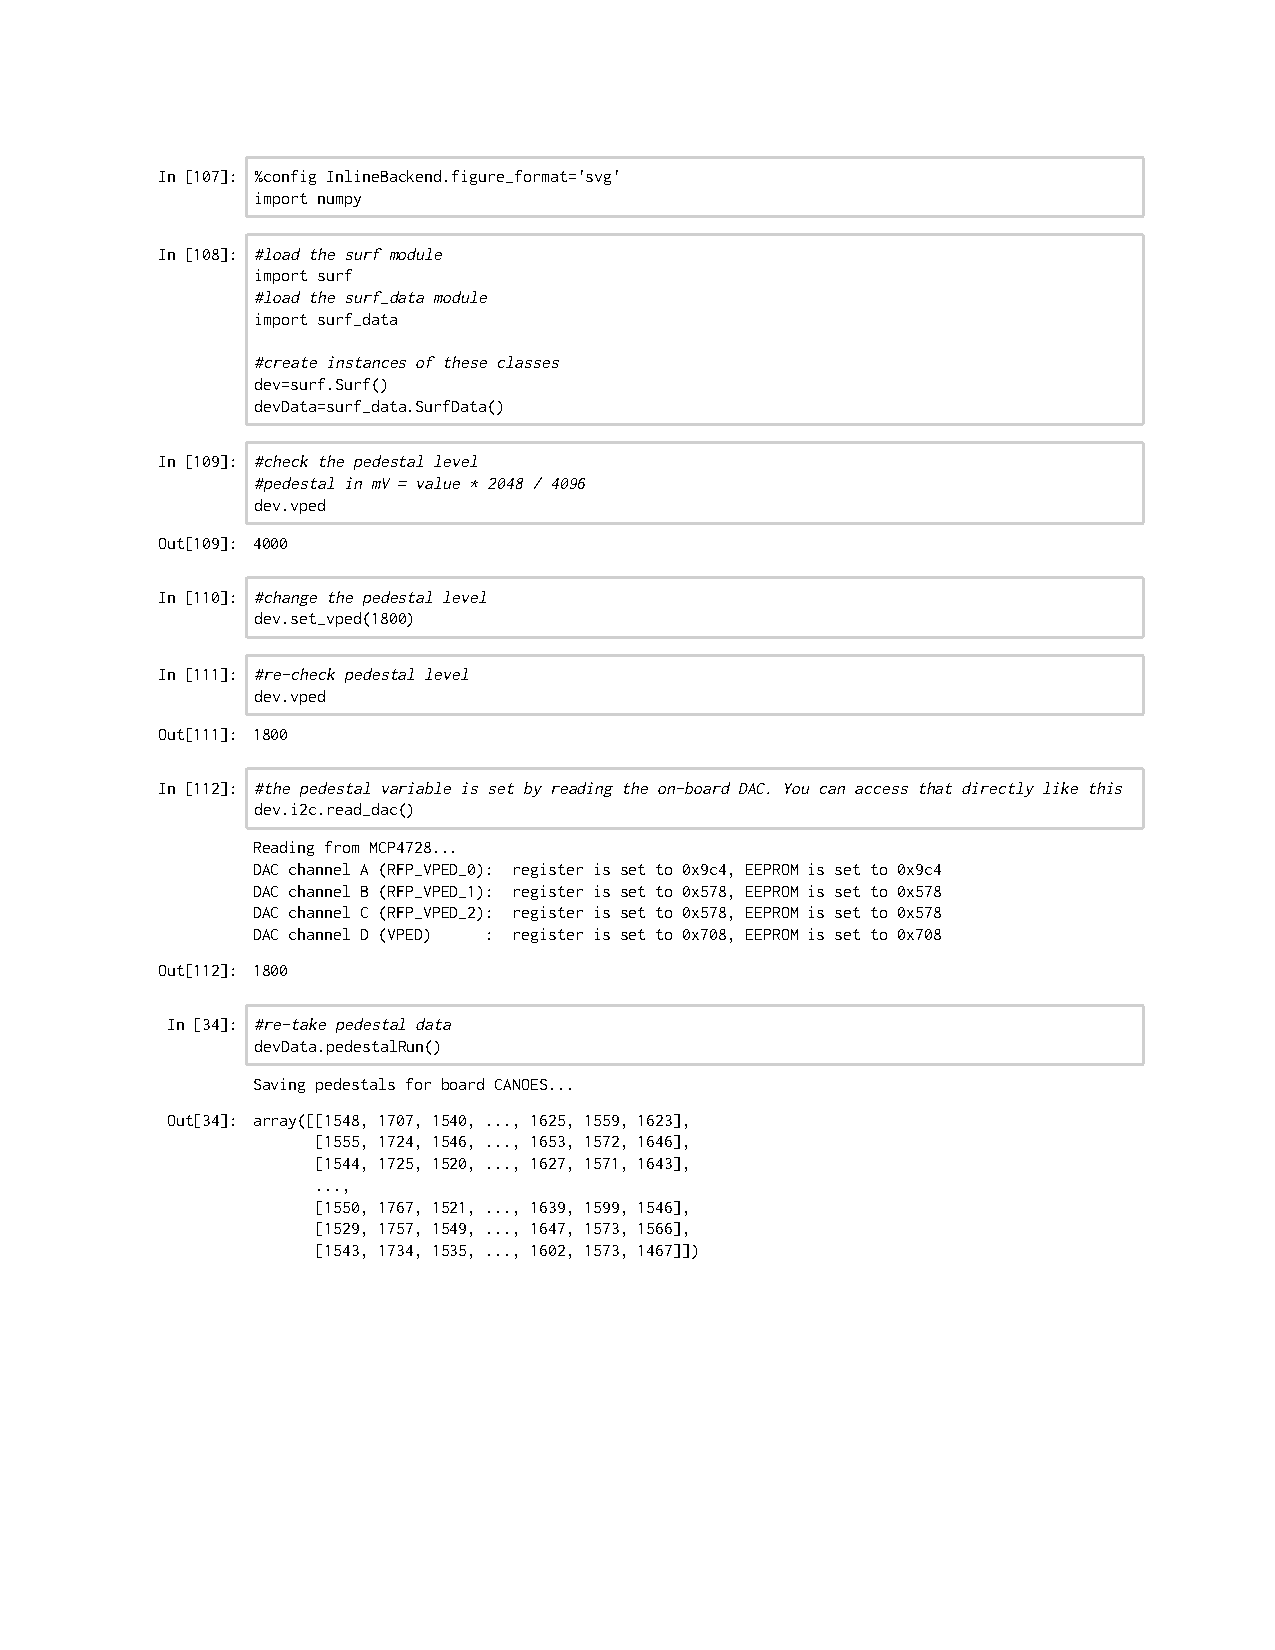
\includepdf[pages={1}, offset=0cm -2cm, pagecommand={\section{IPython Notebook: Basic Operations}\label{Appendix1}}]{fig/surf_ipython.pdf}
\includepdf[pages=2-, offset=0cm -2cm, pagecommand={}]{fig/surf_ipython.pdf}

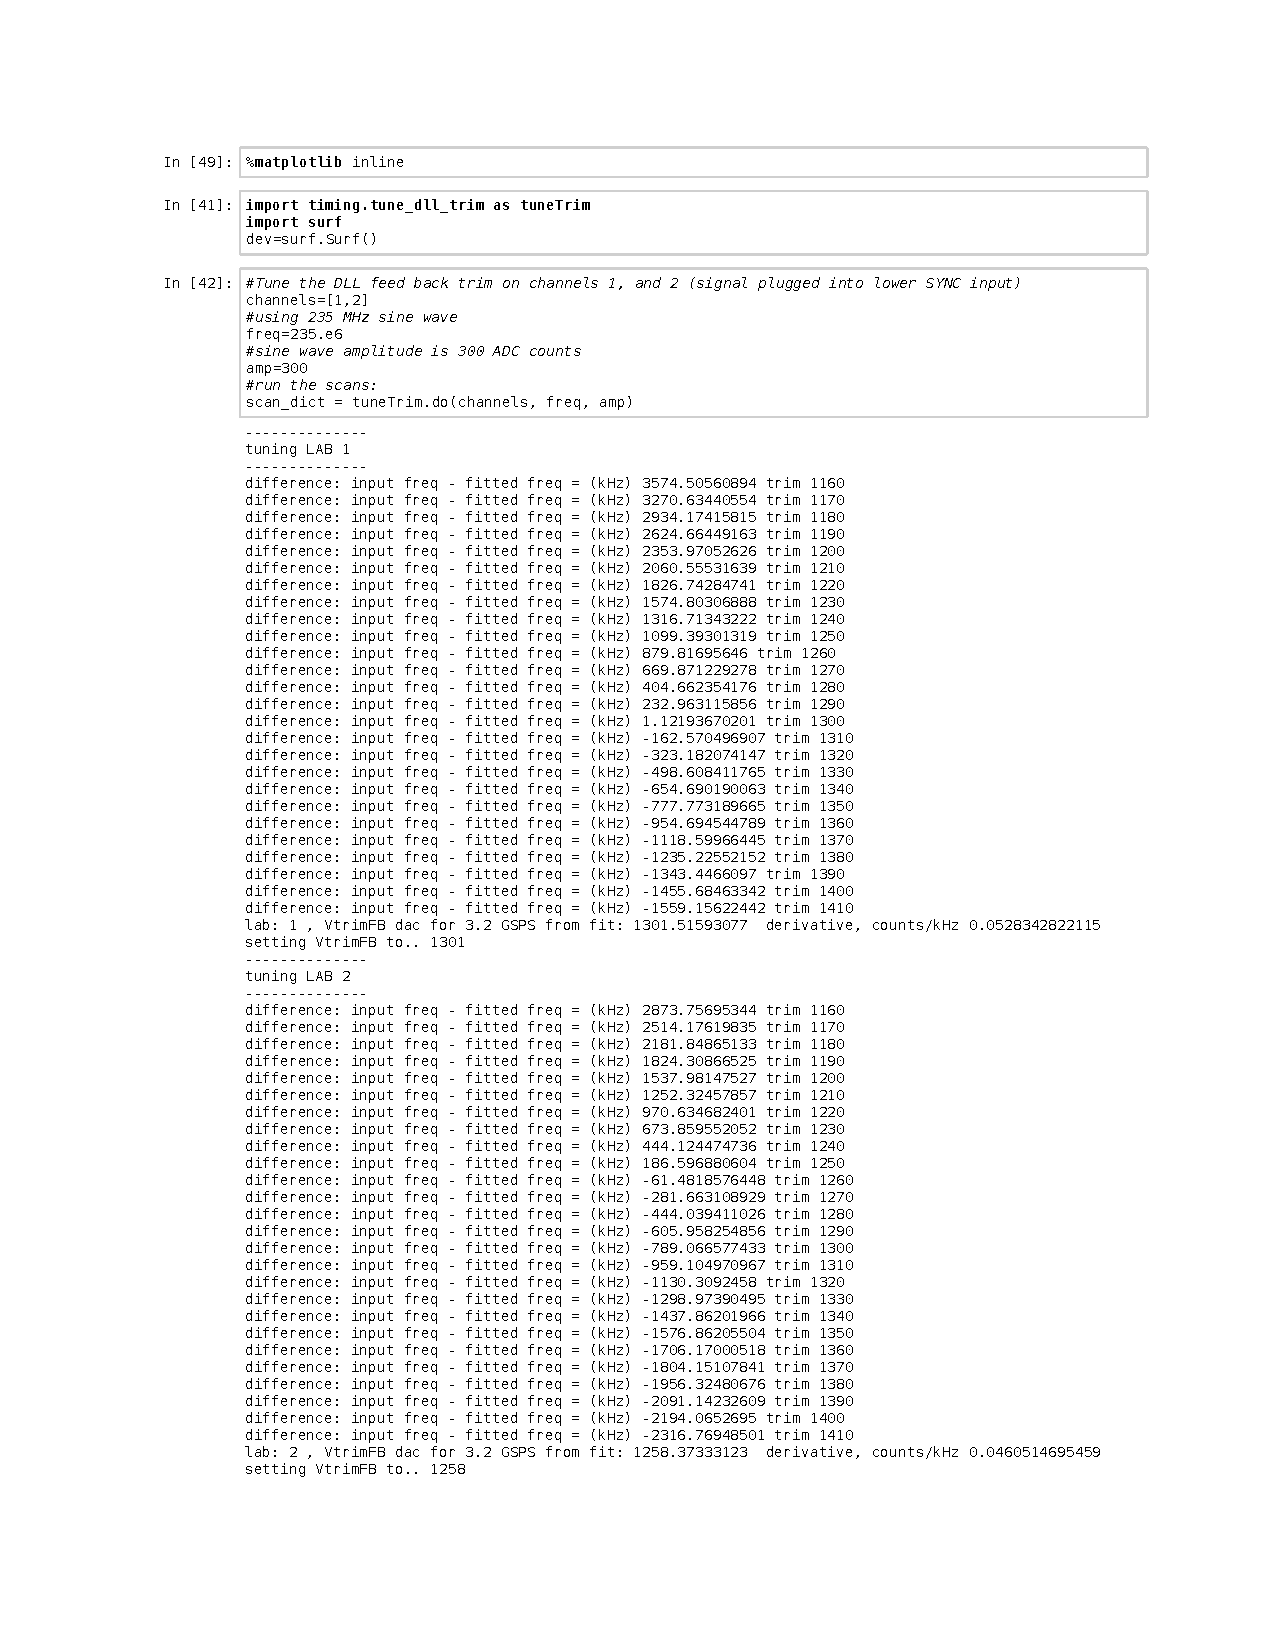
\includepdf[pages={1}, offset=0cm -1cm, pagecommand={\section{IPython Notebook: Tuning DLL feedback trim}\label{Appendix2}}]{fig/vtrimfb_notebook.pdf}
\includepdf[pages={2-}, offset=0cm -1cm, pagecommand={}]{fig/vtrimfb_notebook.pdf}

\end{document}
